\subsection{Messages}\label{sec:messages}
Bon, c'est bien beau mais vous avez peut-être remarqué un gros inconvénient de notre système: lorsqu'un post est créé et qu'il manque un champ, rien ne nous dit clairement le problème! De plus, il serait profitable d'avoir une confirmation lorsqu'un post est créé/modifié/suprimé. C'est exactement à cela que vont servir les variables \verb|'success'| que nous avons créées dans la section précédente, sans les utiliser.

Créez donc un fichier \verb|resources/views/inc/messages.blade.php| et remplissez le comme sur la figure de droite.

\begin{wrapfigure}[8]{r}{0.5\textwidth}
    \vspace{-0.5cm}
    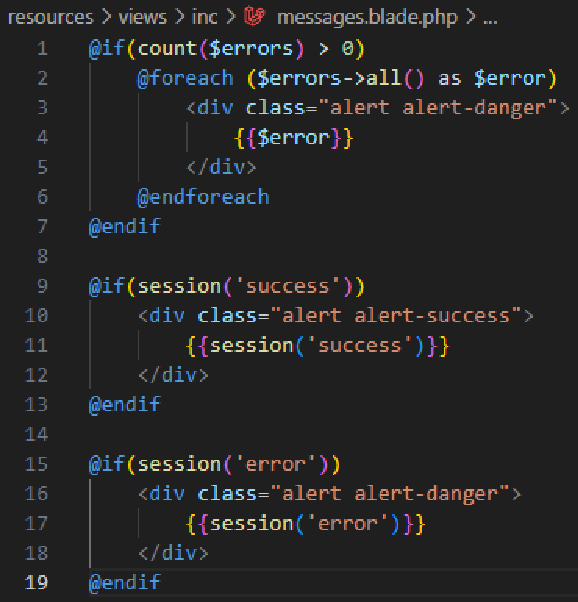
\includegraphics[width=0.5\textwidth]{figures-C1/messages_blade.pdf}
\end{wrapfigure}
Ici, les deuxième et troisième \verb|@if()| permettent de voir si la \verb|session| ($\Rightarrow$ la page actuelle, en gros) possède les variables \verb|'success'| et \verb|'error'|, et de les afficher. 

Ces variables sont celles que nous avons créées \\ aux \texttt{Section~\ref{sec:posts_store},~\ref{sec:posts_update},~\ref{sec:posts_delete}}

Enfin, le premier \verb|@if()| est utilisé afin d'afficher toutes les erreurs provenants d'un fail de validation après la soumission des \verb|<form>|.

\vspace{4cm}

Enfin, voici le résultat que vous devriez obtenir lorsque, par exemple, un post est créé (\textsc{Figure~\ref{fig:messages_create}}) ou lorsque le champ du message n'est pas rempli (\textsc{Figure~\ref{fig:messages_error}}):

\begin{figure}[!h]
    \begin{subfigure}[c]{0.42\textwidth}
        \fbox{
\includegraphics[width=\textwidth]{figures-C1/messages_create.pdf}}
        \caption{\label{fig:messages_create}}
    \end{subfigure}
    \hspace{0.2cm}
    \begin{subfigure}[c]{0.52\textwidth}
        \fbox{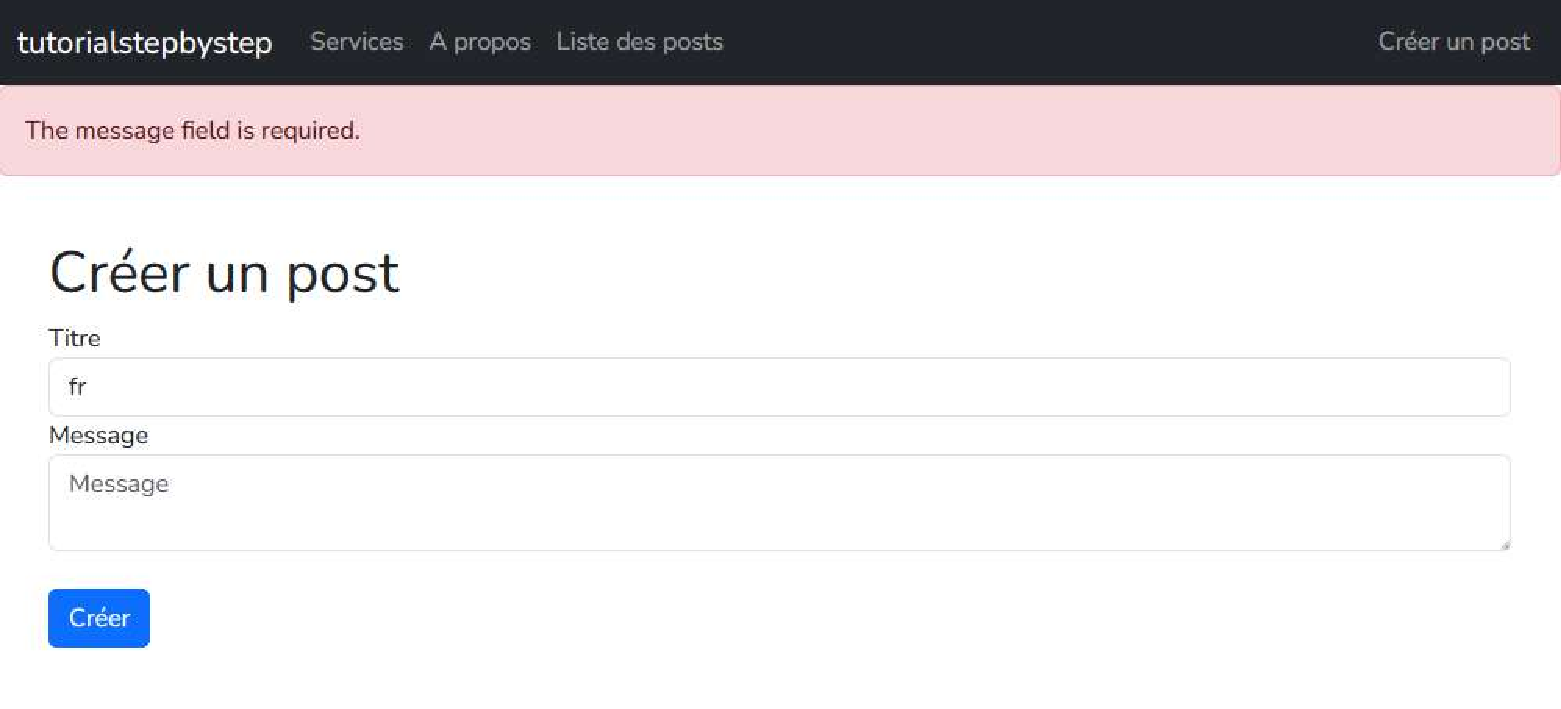
\includegraphics[width=\textwidth]{figures-C1/messages_error.pdf}}
        \caption{\label{fig:messages_error}}
    \end{subfigure}
    \caption{}
\end{figure}

Vous pouvez avoir l'impression que nous en avons enfin fini avec cette formation, mais\ldots il reste quelque chose qui devrait vous chiffoner: Les deux boutons \verb|login| et \verb|register| sur notre page d'accueil, ils ne servent toujours à rien. 

Dans la \texttt{Section~\ref{sec:auth}}, nous allons donc ajouter un système d'authentification très simple à notre site.
